%%%%%%%%%%%%%%%%%%%%%%%%%%%%%%%%%%%%%%%%%%%%%%%%%%%%%%%%%%%%%%%%%%%%%%%%%%%%%%%%%%%%%%%%%%%%%%
%
%   GERMAN
%
%%%%%%%%%%%%%%%%%%%%%%%%%%%%%%%%%%%%%%%%%%%%%%%%%%%%%%%%%%%%%%%%%%%%%%%%%%%%%%%%%%%%%%%%%%%%%%

\title{\textbf{\rmfamily Einführungsvortrag}}
\subtitle{\horrorfont Das Standardmodell der Teilchenphysik und der LHCb Detektor}
\author[~\WorkGroup~]{{\WorkGroup\inst{1}}}
\institute[\WorkGroup]{\inst{1} \University}

%%%%%%%%%%%%%%%%%%%%%%%%%%%%%%%%%%%%%%%%%%%%%%%%%%%%%%%%%%%%%%%%%%%%%%%%%%%%%%%%%%%%%%%%%%%%%%
%   Options for the footline
%%%%%%%%%%%%%%%%%%%%%%%%%%%%%%%%%%%%%%%%%%%%%%%%%%%%%%%%%%%%%%%%%%%%%%%%%%%%%%%%%%%%%%%%%%%%%%
\setbeamertemplate{footline}
{
\leavevmode%
\hbox{%
\begin{beamercolorbox}[wd=0.5\paperwidth,ht=2.25ex,dp=1ex,center]{author in foot}%
\usebeamerfont{author in foot}
\end{beamercolorbox}%
\begin{beamercolorbox}[wd=0.11\paperwidth,ht=2.25ex,dp=1ex,center]{title in head/foot}%
\usebeamerfont{title in head/foot}
\end{beamercolorbox}%
\begin{beamercolorbox}[wd=0.385\paperwidth,ht=2.25ex,dp=1ex,right]{date in head/foot}%
\usebeamerfont{date in head/foot}\insertsection{}\hfill
|~Folie \insertframenumber{} \hspace*{2ex}%/ \inserttotalframenumber\hspace*{2ex}
\end{beamercolorbox}}%
\vskip0pt%
}

%%%%%%%%%%%%%%%%%%%%%%%%%%%%%%%%%%%%%%%%%%%%%%%%%%%%%%%%%%%%%%%%%%%%%%%%%%%%%%%%%%%%%%%%%%%%%%
% Options for the timetable
%%%%%%%%%%%%%%%%%%%%%%%%%%%%%%%%%%%%%%%%%%%%%%%%%%%%%%%%%%%%%%%%%%%%%%%%%%%%%%%%%%%%%%%%%%%%%%

\makeatletter
\newcommand{\setcurrtime}[1]{%
  \set@time\curr@hour\curr@mins#1\@nil
}
\def\set@time#1#2#3:#4\@nil{%
  \def#1{#3}\def#2{#4}%
}
\newcommand{\currtime}[1][00:00]{%
  \begingroup
  \set@time\new@hour\new@mins#1\@nil
  \count\z@=\curr@mins\relax
  \count\tw@=\curr@hour\relax
  \advance\count\z@\new@mins\relax
  \advance\count\tw@\new@hour\relax
  \ifnum\count\z@>59
    \advance\count\z@-60
    \advance\count\tw@\@ne
  \fi
  % we have to use \count\z@ and \count\tw@ before
  % ending the group and printing the result
  \edef\x{\endgroup\two@digits{\count\tw@}:\two@digits{\count\z@}}\x
}
\makeatother


%%%%%%%%%%%%%%%%%%%%%%%%%%%%%%%%%%%%%%%%%%%%%%%%%%%%%%%%%%%%%%%%%%%%%%%%%%%%%%%%%%%%%%%%%%%%%%
%%%%%%%%%%%%%%%%%%%%%%%%%%%%%%%%%%%%%%%%%%%%%%%%%%%%%%%%%%%%%%%%%%%%%%%%%%%%%%%%%%%%%%%%%%%%%%

\begin{document}
\StartMasterclass

%%%%%%%%%%%%%%%%%%%%%%%%%%%%%%%%%%%%%%%%%%%%%%%%%%%%%%%%%%%%%%%%%%%%%%%%%%%%%%%%%%%%%%%%%%%%%%
\begin{frame}{\small \hfill \textcolor{lightgreen}{$\pi=3$}}
\, \vspace{0.1cm}  \Large  \begin{center}
    \textbf{Herzlich Willkommen zur Masterclass!} 
\end{center} 
  \small \, \vspace{1cm} \\
    \emph{Gedulden Sie sich noch ein wenig. Die Veranstaltung beginnt in Kürze.}
\end{frame}
%%%%%%%%%%%%%%%%%%%%%%%%%%%%%%%%%%%%%%%%%%%%%%%%%%%%%%%%%%%%%%%%%%%%%%%%%%%%%%%%%%%%%%%%%%%%%%
\section{}
%%%%%%%%%%%%%%%%%%%%%%%%%%%%%%%%%%%%%%%%%%%%%%%%%%%%%%%%%%%%%%%%%%%%%%%%%%%%%%%%%%%%%%%%%%%%%%
\begin{frame}
\begin{minipage}[t]{0.4\textwidth}
    \includegraphics[width=\textwidth]{Figures Introductory Lecture/Introduction/Human.png}
\end{minipage}
\begin{minipage}[t]{0.55\textwidth}
   \vspace{-3cm} \centering
     \Large{ \textbf{Woraus bestehen eigentlich Menschen?}} \\ \vspace{0.5cm} \normalsize{Und,} \\ \Large \textbf{woher wissen wir das?} % Meldung der SuS sammeln 
\end{minipage}  
\end{frame}
%%%%%%%%%%%%%%%%%%%%%%%%%%%%%%%%%%%%%%%%%%%%%%%%%%%%%%%%%%%%%%%%%%%%%%%%%%%%%%%%%%%%%%%%%%%%%%
\begin{frame}
    \begin{center}
    \Large \textbf{Woraus besteht die Welt?} \\
    \vspace{1cm}
   \textbf{Warum ist sie so gebaut, wie sie es ist?}\\
     \vspace{1cm}
        \large Wir möchten heute der Frage nachgehen: \\ 
    \Large  \textbf{Was ist Materie, wie kann man sie "messen"?}
    \end{center}
    \end{frame}

%%%%%%%%%%%%%%%%%%%%%%%%%%%%%%%%%%%%%%%%%%%%%%%%%%%%%%%%%%%%%%%%%%%%%%%%%%%%%%%%%%%%%%%%%%%%%%

\begin{frame}[plain]
\begin{center}
    \begin{tabular}{ccc}
 \parbox{0.33\textwidth}{\LogoInsitute}    &
 ~~~~\parbox{0.33\textwidth}{\includegraphics[height=1cm]{Logos And Group/LHCb_Logo.png}}   &  \parbox{0.33\textwidth}{\LogoUniversity}\\
\end{tabular}
\end{center}

\maketitle
\end{frame}
%%%%%%%%%%%%%%%%%%%%%%%%%%%%%%%%%%%%%%%%%%%%%%%%%%%%%%%%%%%%%%%%%%%%%%%%%%%%%%%%%%%%%%%%%%%%%%

\GroupPresentation \addtocounter{framenumber}{1}

%%%%%%%%%%%%%%%%%%%%%%%%%%%%%%%%%%%%%%%%%%%%%%%%%%%%%%%%%%%%%%%%%%%%%%%%%%%%%%%%%%%%%%%%%%%%%%
\begin{frame}{Wer seid ihr?}
\Large Wer sind wir? \ding{52} \\ \vspace{1cm}
    \Large Wer seid ihr? \\
    \large ~ \ding{43} Anwesenheitsbogen
\end{frame}
%%%%%%%%%%%%%%%%%%%%%%%%%%%%%%%%%%%%%%%%%%%%%%%%%%%%%%%%%%%%%%%%%%%%%%%%%%%%%%%%%%%%%%%%%%%%%%
\begin{frame}{\textbf{Was ist Materie, wie kann man sie "messen" ?}}
\begin{center}
    \Large Was müssen wir alles wissen, um dieser Frage nachzugehen?  
    % unglücklich formuliert. 
\end{center}
\end{frame}
%%%%%%%%%%%%%%%%%%%%%%%%%%%%%%%%%%%%%%%%%%%%%%%%%%%%%%%%%%%%%%%%%%%%%%%%%%%%%%%%%%%%%%%%%%%%%%
\begin{frame}{Der heutige Tag}

\footnotesize
    \begin{tabular}{rl l}
       \currtime  & Einführungsvortrag & (\PersonIntroductory)\\ 
        \currtime[01:00]   & Anwendung Detektoren &\\
       \currtime[01:45]  & Hadronen. Vortrag und Anwendung; & (\PersonHadrons)  \\
        \currtime[02:45]   & ~~~ \emph{Mittagspause} & \\
        \currtime[03:45] & Datenanalyse. Vortrag und Anwendung & (\PersonDataAnalysis)\\
        \currtime[04:45] & Ergebnisdiskussion &  (\PersonDiscusion)\\
       \currtime[05:00] & Ende& 
    \end{tabular} \\ \, \\
    Pausen gibt es zwischendurch, je nach Bedarf. \\ 
    \ding{43} Auf Toilette dürft immer gehen, ohne zu fragen, \\
    \ding{43} Fragen über Physik dürfen immer gestellt werden!

\end{frame}
%%%%%%%%%%%%%%%%%%%%%%%%%%%%%%%%%%%%%%%%%%%%%%%%%%%%%%%%%%%%%%%%%%%%%%%%%%%%%%%%%%%%%%%%%%%%%%
\section{Einführung in die Teilchenphysik}
%%%%%%%%%%%%%%%%%%%%%%%%%%%%%%%%%%%%%%%%%%%%%%%%%%%%%%%%%%%%%%%%%%%%%%%%%%%%%%%%%%%%%%%%%%%%%%
\begin{frame}[plain]
   \begin{center} 
  \huge{  \ding{182} }\\
   \Large{Einführung in die Teilchenphysik}
\end{center}
\end{frame}
%%%%%%%%%%%%%%%%%%%%%%%%%%%%%%%%%%%%%%%%%%%%%%%%%%%%%%%%%%%%%%%%%%%%%%%%%%%%%%%%%%%%%%%%%%%%%%
\begin{frame}[t]{Und was ist eigentlich im Nukleus?}

    \begin{minipage}{\linewidth}
        \begin{minipage}{0.33\linewidth}
             \qquad Atom 
        \end{minipage}     
        \begin{minipage}{0.3\linewidth}
             \quad Atomkern 
        \end{minipage}    
        \begin{minipage}{0.33\linewidth}
            Proton mit \textbf{Quarks}
        \end{minipage}    
    \end{minipage} \vspace{0.5cm}
    
     \begin{minipage}{0.99\linewidth}
        \begin{figure}
            \centering
            \includegraphics[width=\textwidth]{Figures Introductory Lecture/Standard Model/Scale_Atom_Quark_noText.png}
            \label{fig:scale_atom_qaurk}
        \end{figure}
     \end{minipage}  
     \vspace{-15cm}
    \begin{minipage}{\linewidth}
        \begin{minipage}{0.33\linewidth}
            \qquad \Large $10^{-10}$\,m
        \end{minipage}     
        \begin{minipage}{0.33\linewidth}
             \quad \Large $10^{-15}$\,m
        \end{minipage}    
        \begin{minipage}{0.29\linewidth}
            \quad \Large $\leq10^{-18}$\,m
        \end{minipage}    
    \end{minipage}

\end{frame}
%%%%%%%%%%%%%%%%%%%%%%%%%%%%%%%%%%%%%%%%%%%%%%%%%%%%%%%%%%%%%%%%%%%%%%%%%%%%%%%%%%%%%%%%%%%%%%
\begin{frame}{Quarks - Was sind das?}

    \begin{minipage}[t]{\linewidth}\raggedleft
           Welche Ladung hat ein \textcolor{red}{\textbf{Neutron}}/\textcolor{blue}{\textbf{Proton}}? \\
           Welche Ladung müssen die \textcolor{darkgreen}{\textbf{Q}}\textbf{u}\textcolor{darkgreen}{\textbf{a}}\textbf{r}\textcolor{darkgreen}{\textbf{k}}\textbf{s} haben?
    \end{minipage}%
    \vspace{-0.6cm}
    \begin{minipage}{\linewidth}\raggedright
        \begin{figure}[htb]
            \includegraphics[width=0.79\textwidth]{Figures Introductory Lecture/Standard Model/Quarks.png}
            %\caption{}
            \label{fig:quarks}
        \end{figure}            
    \end{minipage}
    
\end{frame}
%%%%%%%%%%%%%%%%%%%%%%%%%%%%%%%%%%%%%%%%%%%%%%%%%%%%%%%%%%%%%%%%%%%%%%%%%%%%%%%%%%%%%%%%%%%%%%

\begin{frame}{Wie werden Quarks zusammengehalten?}  
    \begin{figure}[htb]
        \includegraphics[width=1\textwidth]{Figures Introductory Lecture/Standard Model/StrongForce_EM.png}
        %\caption{}
        \label{fig:strong_force_1}
    \end{figure} \\
    \Large \begin{center}
        Die Elektromagnetische Kraft \emph{könnte} Quarks binden!
    \end{center}
\end{frame}
%%%%%%%%%%%%%%%%%%%%%%%%%%%%%%%%%%%%%%%%%%%%%%%%%%%%%%%%%%%%%%%%%%%%%%%%%%%%%%%%%%%%%%%%%%%%%%

\begin{frame}{Kräfte in Atomkernen}
...aber warum halten dann \emph{Atomkerne} zusammen?!\\ \, \hspace{2cm} \ding{55} \textcolor{blue}{\textbf{Protonen}} stoßen sich elektromagnetisch ab!

    \begin{figure}[htb]
        \includegraphics[width=0.3\textwidth]{Figures Introductory Lecture/Standard Model/Nukleus.png}
        %\caption{}
        \label{fig:strong_force_2}
    \end{figure}\\
    \ding{43} Es gibt weitere Kraft die Atomkerne bindet\\ 
    \vspace{0.5cm}\begin{center}
    \Large{Die \textbf{Starke Kraft}}
    \end{center}
\end{frame}
%%%%%%%%%%%%%%%%%%%%%%%%%%%%%%%%%%%%%%%%%%%%%%%%%%%%%%%%%%%%%%%%%%%%%%%%%%%%%%%%%%%%%%%%%%%%%%
\begin{frame}{Fragestunde Protonen}
\begin{center} \Large
        ...aber, \\ wie können wir feststellen, ob Protonen nun von der\\ starken oder elektromagnetischen Kraft \\zusammengehalten werden? 
\end{center}

\end{frame}
%%%%%%%%%%%%%%%%%%%%%%%%%%%%%%%%%%%%%%%%%%%%%%%%%%%%%%%%%%%%%%%%%%%%%%%%%%%%%%%%%%%%%%%%%%%%%%
\begin{frame}{Andere Quarkkombinationen}
Tatsächlich finden wir Teilchen, die aus drei  up-Quarks/drei down-Quarks bestehen!
    \begin{figure}[htb]
        \includegraphics[width=0.6\textwidth]{Figures Introductory Lecture/Standard Model/DeltaBaryons.png}
        \label{fig:strong_force_2}
    \end{figure}
    $\hspace{3cm}\rightarrow \Delta^{++}$\hspace{3cm} $\rightarrow \Delta^{-}$\\ \vspace{0.5cm}
    \ding{43} Die \textbf{Starke Kraft} muss für die Bindung verantwortlich sein!
\end{frame}
%%%%%%%%%%%%%%%%%%%%%%%%%%%%%%%%%%%%%%%%%%%%%%%%%%%%%%%%%%%%%%%%%%%%%%%%%%%%%%%%%%%%%%%%%%%%%%
\begin{frame}{Unterschiede der Kräfte}
Wie unterscheiden sich die elektromagnetische und die starke Kraft?
\pause
\begin{itemize}
    \item Wir spüren die starke Kraft nicht im Alltag
    \item Die starke Kraft wirkt anziehend auf elektrisch neutrale \& geladene Teilchen
    \item ...
    \item[\ding{62}] Wir verstehen die elektromagnetische Kraft, bei der Starken Kraft tun wir uns schwerer!
\end{itemize}
\end{frame}
%%%%%%%%%%%%%%%%%%%%%%%%%%%%%%%%%%%%%%%%%%%%%%%%%%%%%%%%%%%%%%%%%%%%%%%%%%%%%%%%%%%%%%%%%%%%%%
\begin{frame}{Die Eigenschaften der starken Wechselwirkung} 
Für die \textbf{Starke Kraft} existiert eine \textbf{Ladung}, auf die sie wirkt! \\
\begin{itemize}
\begin{itemize}
    \item [\ding{220}] Quarks müssen eine sog. \textbf{Farbladung} besitzen\\
    \item[] Teilchen, die wir beobachten, sind aber farblos! \\
    \end{itemize}
   \item[] \textbf{Analogie:}
\end{itemize} \vspace{-0.5cm}
    \begin{figure}[htb]                                                 
    \includegraphics[width=0.8\textwidth]{Figures Introductory Lecture/Standard Model/GrayAdditiveColours.png}                                                                
    \label{fig:strong_force_3}                                         
    \end{figure} \vspace{-0.5cm}
    \ding{220} Insgesamt farbneutrale Teilchen!
\end{frame} 
%%%%%%%%%%%%%%%%%%%%%%%%%%%%%%%%%%%%%%%%%%%%%%%%%%%%%%%%%%%%%%%%%%%%%%%%%%%%%%%%%%%%%%%%%%%%%%
\begin{frame}{Das Standard Modell der Teilchenphysik}
\foreach \n in {1,...,4}{
    \includegraphics<\n>[width=0.9\textwidth]{Figures Introductory Lecture/Standard Model/SM_\n.png}%
}
%%%%%%%%%%%%%%%%%%%%%%%%%%%%%%%%%%%%%%%%%%%%%%%%%%%%%%%%%%%%%%%%%%%%%%%%%%%%%%%%%%%%%%%%%%%%%%
\end{frame}
\begin{frame}{Das Standard Modell der Teilchenphysik}
    \includegraphics[width=0.9\textwidth]{Figures Introductory Lecture/Standard Model/SM2_1.png}
\end{frame}
%%%%%%%%%%%%%%%%%%%%%%%%%%%%%%%%%%%%%%%%%%%%%%%%%%%%%%%%%%%%%%%%%%%%%%%%%%%%%%%%%%%%%%%%%%%%%%

\begin{frame}{Die schwache Wechselwirkung}
\only<1>{
\begin{figure}[htb]
    \includegraphics[width=0.9\textwidth]{Figures Introductory Lecture/Standard Model/LambdaDecay.png}%
   \label{fig:LambdaToProton}
\end{figure}
}
\only<2>{
\begin{figure}[htb]
    \includegraphics[width=0.9\textwidth]{Figures Introductory Lecture/Standard Model/LambdaDecayCharge.png}%
    \label{fig:Lambda_Decay}
\end{figure}
}
\only<3>{
\begin{figure}[htb]
    \includegraphics[width=0.9\textwidth]{Figures Introductory Lecture/Standard Model/LambdaDecayFull.png}%
     \label{fig:Lambda_DecayFull}
\end{figure}
}
\end{frame}
%%%%%%%%%%%%%%%%%%%%%%%%%%%%%%%%%%%%%%%%%%%%%%%%%%%%%%%%%%%%%%%%%%%%%%%%%%%%%%%%%%%%%%%%%%%%%%
\begin{frame}{Feynman Diagramme}
\begin{center}
\begin{tikzpicture}
\begin{feynman}
    \vertex(ul) {\(u\)};
    \vertex[right=5cm of ul] (ur) {\(u\)};
    \vertex[below=0.75cm of ul] (dl) {\(d\)};
    \vertex[right=5cm of dl] (dr) {\(d\)};
    \vertex[below=0.75cm of dl] (sl) {\(s\)};
    \vertex[right=5cm of sl] (ur2) {\(u\)};
    \vertex[right=2cm of sl] (W1);
    \vertex[below right = 1cm and 1.5cm of W1] (W2);
    \vertex[below = 0.5cm of ur2] (e) {\(e^-\)};
    \vertex[below = 1cm of e] (nue) {\(\bar \nu_e\)};
    \diagram* { {[edges=fermion]
    (ul) -- (ur), (dl) -- (dr), (sl) -- (ur2),
    (W2) -- (e), (nue) -- (W2)};
    (W1) -- [boson, edge label' = \(W^-\)] (W2)
    };
\draw [decoration={brace}, decorate]  (sl.south west) -- (ul.north west) node [pos=0.5, left] {\(\Lambda^0\)};
\draw [decoration={brace}, decorate] (ur.north east) --  (ur2.south east) node [pos=0.5, right] {\(p^+\)};
\end{feynman}
\end{tikzpicture}   
\end{center}
\ding{43} Nur die schwache Wechselwirkung ist in der Lage den \textbf{Flavour} eines Teilchens zu verändern! 
\end{frame}
%%%%%%%%%%%%%%%%%%%%%%%%%%%%%%%%%%%%%%%%%%%%%%%%%%%%%%%%%%%%%%%%%%%%%%%%%%%%%%%%%%%%%%%%%%%%%%%

\begin{frame}[fragile]{Das Standard Modell der Teilchenphysik II}
\foreach \n in {1,...,9}{
        \includegraphics<\n>[width=0.9\textwidth]{Figures Introductory Lecture/Standard Model/SM2_\n.png}%
} 
%%%%%%%%%%%%%%%%%%%%%%%%%%%%%%%%%%%%%%%%%%%%%%%%%%%%%%%%%%%%%%%%%%%%%%%%%%%%%%%%%%%%%%%%%%%%%%
\end{frame}
\begin{frame}{Standard Modell: Das wichtigste für heute}
\begin{itemize} \Large
    \item[\ding{55}] 6 Quark-Flavours  $u$, $d$, $c$, $s$, $b$, $t$
    \item[\ding{55}] Starke-, Schwache- und Elektromagnetische Kraft
    \item[\ding{55}] Flavour-Änderung nur über Schwachen Zerfall
    \item[\ding{55}] Austauschteilchen $\gamma$, $Z^0$ \& $W^{\pm}$, $g$
    \item[\ding{55}] Farbladung als Ladung der Starken Kraft
    \item[\ding{55}] Quarks farbig, Teilchen farbneutral
    \item[\ding{62}] Starke Kraft recht unverstanden!
\end{itemize}
    
\end{frame}
%%%%%%%%%%%%%%%%%%%%%%%%%%%%%%%%%%%%%%%%%%%%%%%%%%%%%%%%%%%%%%%%%%%%%%%%%%%%%%%%%%%%%%%%%%%%%%
  \begin{frame}{Was ist Materie, wie kann man sie "messen"?}\Large
 Und jetzt?
 \begin{itemize}
     \item Wie kann man Teilchen erzeugen?
     \item Wie können wir das alles nachweisen?!
 \end{itemize}
\begin{center} \pause
 
Aber erstmal \\   \textbf{\textcolor{red}{5\,min Pause :)}
}
\end{center}  
\end{frame}
%%%%%%%%%%%%%%%%%%%%%%%%%%%%%%%%%%%%%%%%%%%%%%%%%%%%%%%%%%%%%%%%%%%%%%%%%%%%%%%%%%%%%%%%%%%%%% 
   \section{LHCb-Detektor am CERN}
\begin{frame}[plain]

\begin{center} 
  \huge{  \ding{183} }\\
   \Large{ Einführung in den LHCb-Detektor am CERN}

\end{center}
\end{frame}
%%%%%%%%%%%%%%%%%%%%%%%%%%%%%%%%%%%%%%%%%%%%%%%%%%%%%%%%%%%%%%%%%%%%%%%%%%%%%%%%%%%%%%%%%%%%%%

\begin{frame}{Ein Teilchen bitte!}

    \begin{center}
   \Large Wir wollen Teilchen produzieren!\\
    
    \Large Dazu brauchen wir viel \textbf{\textcolor{red}{Energie}}!
   \mathrm{ \begin{align*}
        \textcolor{red}{E} = m\cdot c^\textsf{2} 
    \end{align*}
    }
        
    \end{center}
    
\end{frame}
%%%%%%%%%%%%%%%%%%%%%%%%%%%%%%%%%%%%%%%%%%%%%%%%%%%%%%%%%%%%%%%%%%%%%%%%%%%%%%%%%%%%%%%%%%%%%%

\begin{frame}{Willkommen am CERN \& LHC}

  \begin{center}
   \Large Wie kann man die benötigte Energie bereitstellen?
    \end{center}
    
    \begin{figure}[h]
        \centering
        \includegraphics[width=0.7\textwidth]{Figures Introductory Lecture/LHCb Detector/LHC.jpg} % https://visit.cern/node/616
        \label{fig:CERN_LHC}
    \end{figure}
\end{frame}

%%%%%%%%%%%%%%%%%%%%%%%%%%%%%%%%%%%%%%%%%%%%%%%%%%%%%%%%%%%%%%%%%%%%%%%%%%%%%%%%%%%%%%%%%%%%%%
\begin{frame}
\begin{figure}
\includegraphics[width=\textwidth]{Figures Introductory Lecture/LHCb Detector/LHC.jpg}
\end{figure}
\end{frame}
%%%%%%%%%%%%%%%%%%%%%%%%%%%%%%%%%%%%%%%%%%%%%%%%%%%%%%%%%%%%%%%%%%%%%%%%%%%%%%%%%%%%%%%%%%%%%%
\begin{frame}\addtocounter{framenumber}{-1}
\begin{figure}
\includegraphics[width=\textwidth]{Figures Introductory Lecture/LHCb Detector/LHC+GVA_DE.jpg}
\end{figure}
\end{frame}
%%%%%%%%%%%%%%%%%%%%%%%%%%%%%%%%%%%%%%%%%%%%%%%%%%%%%%%%%%%%%%%%%%%%%%%%%%%%%%%%%%%%%%%%%%%%%%
\begin{frame}\addtocounter{framenumber}{-1}
\begin{figure}
\includegraphics[width=\textwidth]{Figures Introductory Lecture/LHCb Detector/LHC+GVA+TGV_DE.jpg}
\end{figure}
\end{frame}
%%%%%%%%%%%%%%%%%%%%%%%%%%%%%%%%%%%%%%%%%%%%%%%%%%%%%%%%%%%%%%%%%%%%%%%%%%%%%%%%%%%%%%%%%%%%%%
\begin{frame}{Die Kollision der Teilchen}%{Collision and Detection}
Die hochenergetischen Teilchen kollidieren\\
\ding{55}  Was geschieht mit der Energie? % Energieerhaltung
 \\ 
\begin{figure}[h]
       
       \includegraphics[width=0.55\textwidth]{Figures Introductory Lecture/LHCb Detector/Kollision.png}
        \label{fig:Kollision}
    \end{figure}
\end{frame}
%%%%%%%%%%%%%%%%%%%%%%%%%%%%%%%%%%%%%%%%%%%%%%%%%%%%%%%%%%%%%%%%%%%%%%%%%%%%%%%%%%%%%%%%%%%%%%
\begin{frame}{Detektive für Teilchen}%{LHCb}
Wie können wir feststellen, was bei der Kollision passiert ist?\\
\ \\
    \begin{figure}[h]
       
        \includegraphics[width=0.8\textwidth]{Figures Introductory Lecture/LHCb Detector/Detectorsignal_DE.png}
        \label{fig:Detektorsignal}
    \end{figure}

    \begin{itemize}
        \item<2->[\ding{55}] Welches Signal gehört zu welchem Teilchen?
    \end{itemize}
    
\end{frame}
%%%%%%%%%%%%%%%%%%%%%%%%%%%%%%%%%%%%%%%%%%%%%%%%%%%%%%%%%%%%%%%%%%%%%%%%%%%%%%%%%%%%%%%%%%%%%%
\begin{frame}{Welches Signal gehört zu welchem Teilchen?}
    

\ \\
Erinnert euch an die Eigenschaften der Teilchen, die ihr kennt: \\
\begin{itemize}
    \item<2-> Masse \hfill $m$ \hspace{6cm}\,
    \item<2-> Elektrische Ladung  \hfill $q$ \hspace{6cm}\,
    \item<2-> Energie  \hfill $E$ \hspace{6cm}\,
    \item<2-> Impuls  \hfill $\vec{p} $ \hspace{6cm}\,
    \item<2-> Geschwindigkeit  \hfill $\vec{v}$ \hspace{6cm}\,
 
\ \\
    \item<3->[\ding{220}] Wie können wir mit dem LHCb-Detektor diese Eigenschaften messen?

    
\end{itemize}
\end{frame}
%%%%%%%%%%%%%%%%%%%%%%%%%%%%%%%%%%%%%%%%%%%%%%%%%%%%%%%%%%%%%%%%%%%%%%%%%%%%%%%%%%%%%%%%%%%%%%
\begin{frame}{Vertex Locator (VELO)}
    \begin{minipage}{0.58\textwidth}
        \begin{itemize}
        \item Um den Kollisionspunkt aufgebaut
        \item Wichtig für Spurrekonstruktion
    \end{itemize}
    \end{minipage}\hfill
    \begin{minipage}{0.38\textwidth}
        \begin{figure}[h]
        \centering
        \includegraphics[height=3 cm]{Figures Introductory Lecture/LHCb Detector/LHCb_VELO.jpg}%source: http://cds.cern.ch/record/1017398
        \end{figure}
    \end{minipage}
    \vspace{-1cm}
    \begin{figure}[h]
    \centering
    \includegraphics[width=0.8\textwidth]{Figures Introductory Lecture/LHCb Detector/LHCb_1_DE.png}
    \end{figure}
\end{frame}
%%%%%%%%%%%%%%%%%%%%%%%%%%%%%%%%%%%%%%%%%%%%%%%%%%%%%%%%%%%%%%%%%%%%%%%%%%%%%%%%%%%%%%%%%%%%%%
\begin{frame}{Ring Imaging Cherenkov Detector (RICH1)}
    \begin{minipage}{0.68\textwidth}
    \begin{itemize}
        \item Misst \textcolor{red}{\textbf{Geschwindigkeit}} der Teilchen
        \item Wichtig für Identifikation von Teilchen
        \item Nur genau in begrenztem Geschwindigkeitsfenster
    \end{itemize}
    \end{minipage}\hfill
    \begin{minipage}{0.28\textwidth}
        \begin{figure}[h]
        \centering
        \includegraphics[height=2.5 cm]{Figures Introductory Lecture/LHCb Detector/LHCb_RICH1.jpeg}%source:https://cds.cern.ch/record/2807064
        \end{figure}
    \end{minipage}
    \vspace{-0.5cm}
    \begin{figure}[h]
    \centering
    \includegraphics[width=0.8\textwidth]{Figures Introductory Lecture/LHCb Detector/LHCb_2_DE.png}
    \end{figure}
\end{frame}
%%%%%%%%%%%%%%%%%%%%%%%%%%%%%%%%%%%%%%%%%%%%%%%%%%%%%%%%%%%%%%%%%%%%%%%%%%%%%%%%%%%%%%%%%%%%%%
\begin{frame}{Tracker Turicensis (TT)}
    \begin{minipage}{0.58\textwidth}
    \begin{itemize}
        \item Misst die \textcolor{red}{\textbf{Position}} der Teilchen
        \item Trägt zur Spurrekonstruktion bei
    \end{itemize}
    \end{minipage}\hfill
    \begin{minipage}{0.38\textwidth}
        \begin{figure}[h]
        \centering
        \includegraphics[height=2.5 cm]{Figures Introductory Lecture/LHCb Detector/LHCb_TT.jpg}%source:https://twiki.cern.ch/twiki/bin/view/LHCb/ConferenceSummaryIEEFlorida2009
        \end{figure}
    \end{minipage}
    \vspace{-0.5cm}
    \begin{figure}[h]
    \centering
    \includegraphics[width=0.8\textwidth]{Figures Introductory Lecture/LHCb Detector/LHCb_3_DE.png}
    \end{figure}
\end{frame}
%%%%%%%%%%%%%%%%%%%%%%%%%%%%%%%%%%%%%%%%%%%%%%%%%%%%%%%%%%%%%%%%%%%%%%%%%%%%%%%%%%%%%%%%%%%%%%
\begin{frame}{Magnet}
    \begin{minipage}{0.58\textwidth}
    \begin{itemize}
        \item Krümmt die Flugbahn der Teilchen proportional zum \textcolor{red}{\textbf{Impuls}} und \textcolor{red}{\textbf{el. Ladung}} 
        \item Hilft Teilchen zu identifizieren %hier evtl. schüler fragen wieso?
    \end{itemize}
    \end{minipage}\hfill
    \begin{minipage}{0.38\textwidth}
        \begin{figure}[h]
        \centering
        \includegraphics[height=2.5 cm]{Figures Introductory Lecture/LHCb Detector/LHCb_Magnet.jpg}%source:https://cds.cern.ch/record/1124307
        \end{figure}
    \end{minipage}
    \vspace{-0.5cm}
    \begin{figure}[h]
    \centering
    \includegraphics[width=0.8\textwidth]{Figures Introductory Lecture/LHCb Detector/LHCb_4_DE.png}
    \end{figure}
\end{frame}
%%%%%%%%%%%%%%%%%%%%%%%%%%%%%%%%%%%%%%%%%%%%%%%%%%%%%%%%%%%%%%%%%%%%%%%%%%%%%%%%%%%%%%%%%%%%%%
\begin{frame}{Tracker T1, T2 und T3}
    \begin{minipage}{0.58\textwidth}
    \begin{itemize}
        \item Misst die \textcolor{red}{\textbf{Position}} der Teilchen
        \item Hilft Teilchen zu identifizieren %hier evtl. schüler fragen wie?
    \end{itemize}
    \end{minipage}\hfill
    \begin{minipage}{0.38\textwidth}
        \begin{figure}[h]
        \centering
        \includegraphics[height=2.5 cm]{Figures Introductory Lecture/LHCb Detector/LHCb_T1-3.jpg} %source:https://www.facebook.com/LHCbExperiment/photos/a.238680152959433/1123439814483458/?type=3
        \end{figure}
    \end{minipage}
    \vspace{-0.5cm}
    \begin{figure}[h]
    \centering
    \includegraphics[width=0.8\textwidth]{Figures Introductory Lecture/LHCb Detector/LHCb_5_DE.png}
    \end{figure}
\end{frame}
%%%%%%%%%%%%%%%%%%%%%%%%%%%%%%%%%%%%%%%%%%%%%%%%%%%%%%%%%%%%%%%%%%%%%%%%%%%%%%%%%%%%%%%%%%%%%%
\begin{frame}{Ring Imaging Cherenkov Detector (RICH2)}
    \begin{minipage}{0.58\textwidth}
    \begin{itemize}
        \item Funktioniert wie RICH1
        \item Nutzt anderes Medium \ding{220} genau in anderem Geschwindigkeitsfenster
    \end{itemize}
    \end{minipage}\hfill
    \begin{minipage}{0.38\textwidth}
        \begin{figure}[h]
        \centering
        \includegraphics[height=2.5 cm]{Figures Introductory Lecture/LHCb Detector/LHCb_RICH2.jpg}%source:https://www.lhc-facts.ch/index.php?page=lhcb dort wird als quelle cern genannt
        \end{figure}
    \end{minipage}
    \vspace{-0.5cm}
    \begin{figure}[h]
    \centering
    \includegraphics[width=0.8\textwidth]{Figures Introductory Lecture/LHCb Detector/LHCb_6_DE.png}
    \end{figure}
\end{frame}
%%%%%%%%%%%%%%%%%%%%%%%%%%%%%%%%%%%%%%%%%%%%%%%%%%%%%%%%%%%%%%%%%%%%%%%%%%%%%%%%%%%%%%%%%%%%%%
\begin{frame}{Elektromagnetisches Kalorimeter (ECAL)}
    \begin{minipage}{0.58\textwidth}
    \begin{itemize}
        \item Stoppt Elektronen und Photonen
        \item Misst deponierte \textcolor{red}{\textbf{Energie}}
    \end{itemize}
    \end{minipage}\hfill
    \begin{minipage}{0.38\textwidth}
        \begin{figure}[h]
        \centering
        \includegraphics[height=2.5 cm]{Figures Introductory Lecture/LHCb Detector/LHCb_ECAL.JPG}%source:https://cds.cern.ch/record/835712
        \end{figure}
    \end{minipage}
    \vspace{-0.5cm}
    \begin{figure}[h]
    \centering
    \includegraphics[width=0.8\textwidth]{Figures Introductory Lecture/LHCb Detector/LHCb_7_DE.png}
    \end{figure}
\end{frame}
%%%%%%%%%%%%%%%%%%%%%%%%%%%%%%%%%%%%%%%%%%%%%%%%%%%%%%%%%%%%%%%%%%%%%%%%%%%%%%%%%%%%%%%%%%%%%%
\begin{frame}{Hadronisches Kalorimeter (HCAL)}
    \begin{minipage}{0.58\textwidth}
    \begin{itemize}
        \item Stoppt auch schwere geladene und neutrale Teilchen
        \item Misst deponierte \textcolor{red}{\textbf{Energie}}
    \end{itemize}
    \end{minipage}\hfill
    \begin{minipage}{0.38\textwidth}
        \begin{figure}[h]
        \centering
        \includegraphics[height=2.5 cm]{Figures Introductory Lecture/LHCb Detector/LHCb_HCAL.jpg}%source:https://www.lhc-facts.ch/index.php?page=lhcb dort wird als quelle cern genannt
        \end{figure}
    \end{minipage}
    \vspace{-0.5cm}
    \begin{figure}[h]
    \centering
    \includegraphics[width=0.8\textwidth]{Figures Introductory Lecture/LHCb Detector/LHCb_8_DE.png}
    \end{figure}
\end{frame}
%%%%%%%%%%%%%%%%%%%%%%%%%%%%%%%%%%%%%%%%%%%%%%%%%%%%%%%%%%%%%%%%%%%%%%%%%%%%%%%%%%%%%%%%%%%%%%
\begin{frame}{Myonenkammern}
    \begin{minipage}{0.58\textwidth}
    \begin{itemize}
        \item Misst \textcolor{red}{\textbf{Position}} von Myonen
    \end{itemize}
    \end{minipage}\hfill
    \begin{minipage}{0.38\textwidth}
        \begin{figure}[h]
        \centering
        \includegraphics[height=2.5 cm]{Figures Introductory Lecture/LHCb Detector/LHCb_Muon.jpg}%source:https://www.lhc-facts.ch/index.php?page=lhcb dort wird als quelle cern genannt
        \end{figure}
    \end{minipage}
    \vspace{-0.5cm}
    \begin{figure}[h]
    \centering
    \includegraphics[width=0.8\textwidth]{Figures Introductory Lecture/LHCb Detector/LHCb_9_DE.png}
    \end{figure}
\end{frame}
%%%%%%%%%%%%%%%%%%%%%%%%%%%%%%%%%%%%%%%%%%%%%%%%%%%%%%%%%%%%%%%%%%%%%%%%%%%%%%%%%%%%%%%%%%%%%%
\begin{frame}{Messbereich von LHCb}
    \begin{figure}[h]
    \centering
    \includegraphics[width=\textwidth]{Figures Introductory Lecture/LHCb Detector/LHCb_10_DE.png}
    \end{figure}
\end{frame}

\begin{frame}{Was macht wo ein Signal?}
\begin{figure}[h]
    \centering
    \includegraphics[width=\textwidth]{Figures Introductory Lecture/LHCb Detector/Energy Depostition LHCb.png}
    %\c%aption{%Caption}
    \label{fig:energy_deposition}
\end{figure}
\end{frame}
%%%%%%%%%%%%%%%%%%%%%%%%%%%%%%%%%%%%%%%%%%%%%%%%%%%%%%%%%%%%%%%%%%%%%%%%%%%%%%%%%%%%%%%%%%%%%%
\begin{frame}{Wie sieht ein gemessenes Ereignis aus?}
\begin{figure}[h]
    \centering
    \includegraphics[width=\textwidth]{Figures Introductory Lecture/LHCb Detector/LHCb_Eventdisplay.png}
   \label{fig:energy_deposition}
\end{figure}
\end{frame}
\begin{frame}{LHCb - Zusammenfassung}
    Erinnert euch an die Eigenschaften der Teilchen, die ihr kennt \\
\begin{table}[]
    \centering
    \begin{tabular}{lcr}
    ~~~~~Eigenschaft&& Subdetektor~~~ \\ \hline 
 Masse & $m$ \,&  ?\, \\
     El. Ladung  & $q$ \,& Magnet, Tracker  \\
     Energie  & $E$ \,& Kalorimenter, Tracker  \\
     Impuls  & $\vec{p} $ \,& ?  \\
     Geschwindigkeit  & $\vec{v}$ \,& RICH, Magnet, Tracker \\ \hline
    \end{tabular} \pause
\end{table}
\ding{220} Spuren müssen mit Trackern rekonstruiert, zu Teilchen zugeordnet werden!\\
\ding{220} Impuls und Masse müssen berechnet (abgeschätzt) werden! \\\pause
  \ding{43} Eure Aufgabe jetzt!
\end{frame}
%%%%%%%%%%%%%%%%%%%%%%%%%%%%%%%%%%%%%%%%%%%%%%%%%%%%%%%%%%%%%%%%%%%%%%%%%%%%%%%%%%%%%%%%%%%%%%
\end{document}
